\chapter{時系列UX評価システムの提案}
\label{chap:sequential}

\section{時系列UX評価システムの設計・開発}

\subsection{時系列ストレスグラフ}

\subsection{観察ビデオとのマッピング}

\section{有用性の実験計画}

2021年11月から12月に49名の大学生を対象に実験を行った.被験者の平均年齢は20.5歳($SD=1.66$),男女の内訳は男子23名,女子26名であった.

\subsection{実験マテリアルの開発}

\begin{figure}[htbp]
  \begin{minipage}{0.5\hsize}
    \begin{center}
       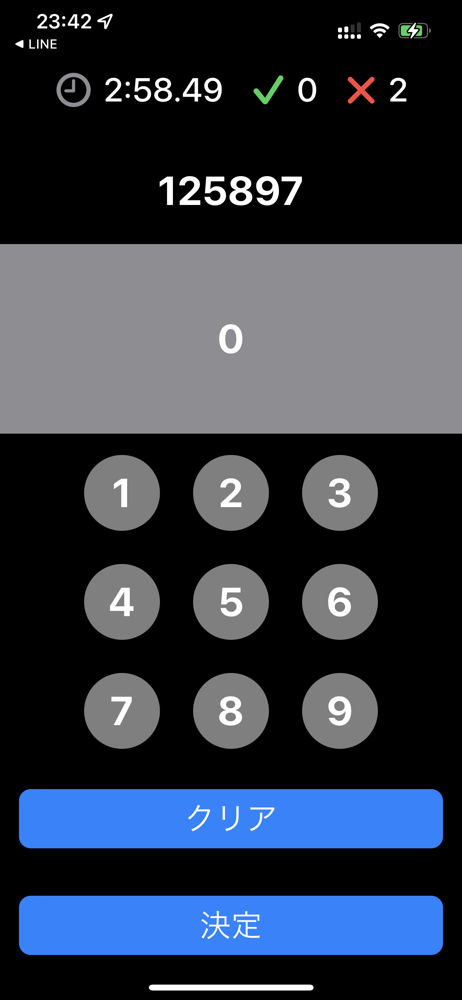
\includegraphics[width=40mm]{img/new1.png}
    \end{center}
    \caption{実験A(テンキー)の画面}
    \label{fig:tenkey}
  \end{minipage}
  \begin{minipage}{0.5\hsize}
    \begin{center}
       
\includegraphics[width=40mm]{img/new2.png}
    \end{center}
    \caption{実験B(ドラッグ)の画面}
    \label{fig:drag}
  \end{minipage}
\end{figure}

\subsection{タスクの実施}

\subsection{容積脈波(BVP)の計測}

\begin{figure}[htbp]
  \begin{minipage}{\hsize}
    \begin{center}
       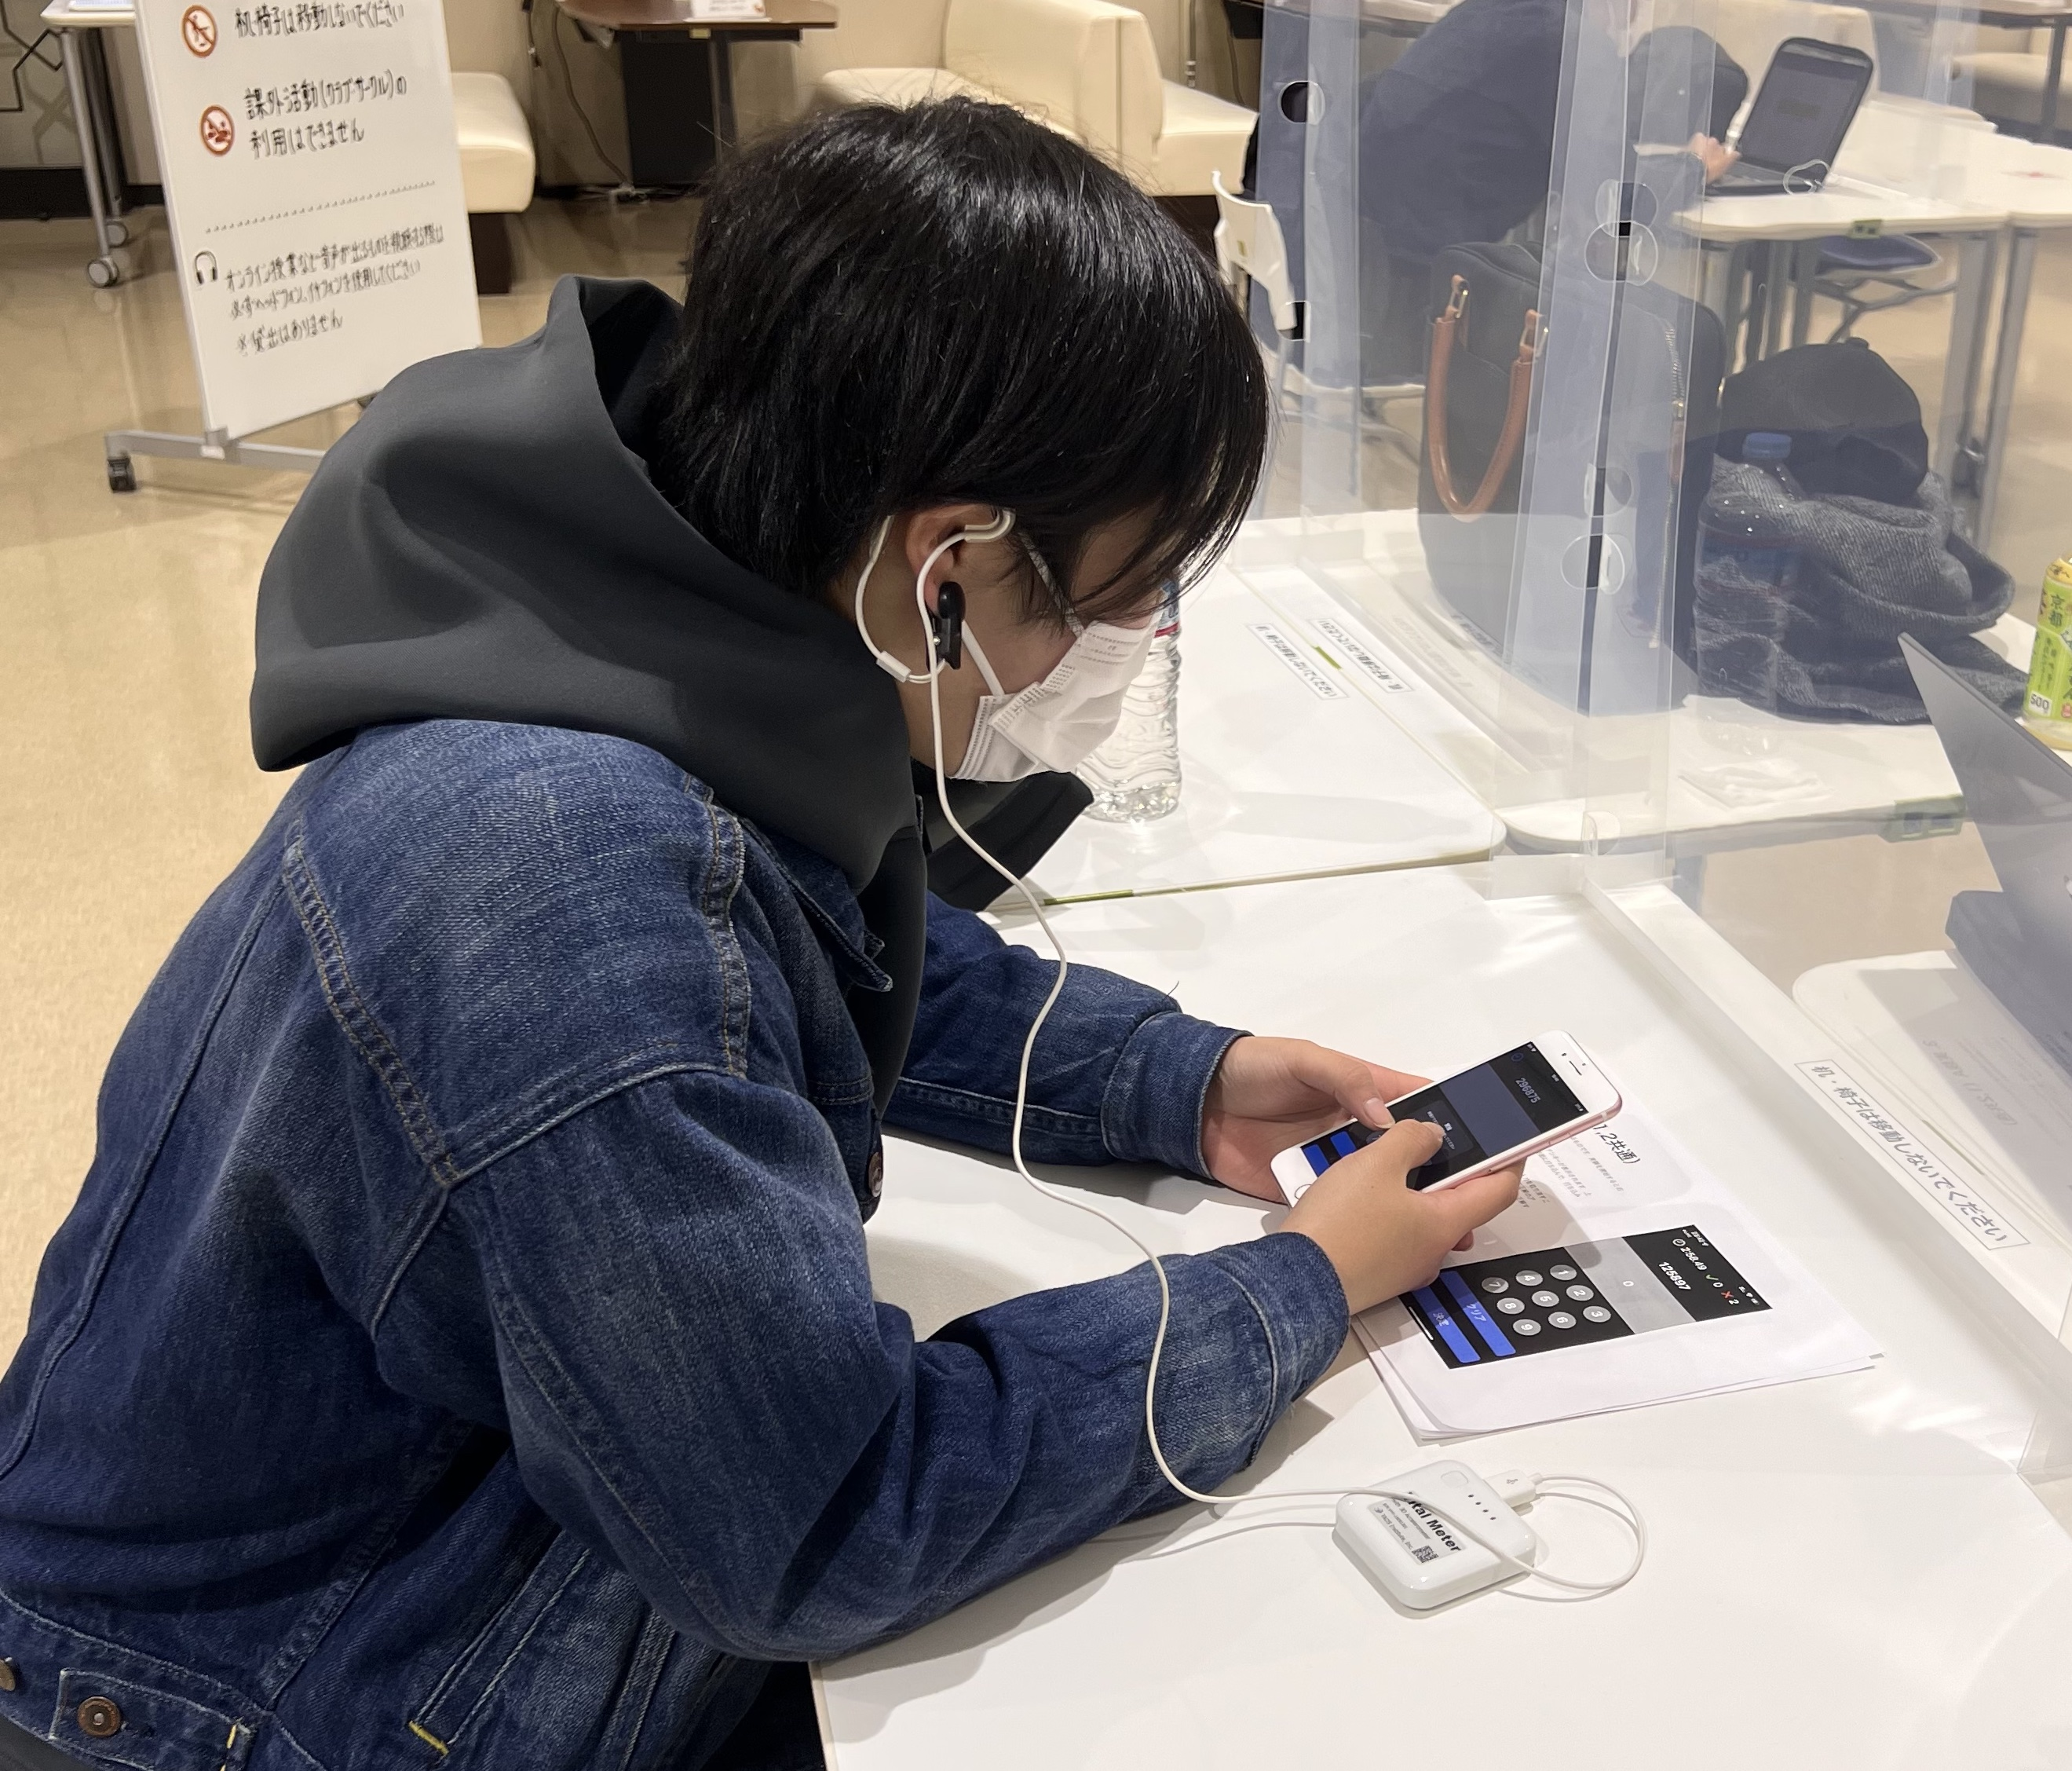
\includegraphics[width=100mm]{img/experience.jpg}
    \end{center}
    \caption{実験の様子}
    \label{fig:observe}
  \end{minipage}
\end{figure}

\subsection{アンケートの実施}

\section{実験の結果}

\section{実験の分析}

\begin{table}[htbp]
\centering
\begin{tabular}{llrlr}
\hline
    & \multicolumn{2}{l}{実験A}                             & \multicolumn{2}{l}{実験B}                             \\ \cline{2-5} 
    & Good UI(件)                & \multicolumn{1}{l}{Bad UI(件)} & Good UI(件)                & \multicolumn{1}{l}{Bad UI(件)} \\ \hline
肯定的 & \multicolumn{1}{r}{16} & 1                          & \multicolumn{1}{r}{22} & 3                          \\
否定的 & \multicolumn{1}{r}{}   & 34                         & \multicolumn{1}{r}{1}  & 34                         \\ \hline
\end{tabular}
\caption{アンケートの自由記述での否定・肯定意見の内訳}
\label{table:negaposi}
\end{table}

\begin{table}[htbp]
\centering
\begin{tabular}{lrrrrr}
\hline
            & \multicolumn{1}{l}{実験A}     & \multicolumn{1}{l}{}       & \multicolumn{1}{l}{実験B}     & \multicolumn{1}{l}{}       & \multicolumn{1}{l}{\multirow{2}{*}{合計(件)}} \\ \cline{2-5}
            & \multicolumn{1}{l}{Good UI(件)} & \multicolumn{1}{l}{Bad UI(件)} & \multicolumn{1}{l}{Good UI(件)} & \multicolumn{1}{l}{Bad UI(件)} & \multicolumn{1}{l}{}                    \\ \hline
スムーズ        & 7                           &                            & 8                           &                            & 15                                      \\
反応が良い       & 3                           &                            & 5                           &                            & 8                                       \\
快適だった       & 3                           &                            & 5                           &                            & 8                                       \\
正常だった       & 2                           &                            & 1                           &                            & 3                                       \\
ゲーム性があった    &                             & 1                          &                             & 1                          & 2                                       \\
達成感があった     &                             &                            &                             & 2                          & 2                                       \\
順調だった       &                             &                            & 2                           &                            & 2                                       \\
ストレスを感じなかった & 1                           &                            & 1                           &                            & 2                                       \\
挑戦したくなった    & 1                           &                            &                             &                            & 1                                       \\
ミスが無かった     &                             &                            & 1                           &                            & 1                                       \\
多く正解できた     & 1                           &                            &                             &                            & 1                                       \\
楽しかった       & 1                           &                            &                             &                            & 1                                       \\ \hline
\end{tabular}
\caption{アンケートの自由記述での肯定的意見の内訳}
\label{table:posi}
\end{table}

\begin{table}[htbp]
\centering
\begin{tabular}{lrrrrr}
\hline
             & \multicolumn{1}{l}{実験A}     & \multicolumn{1}{l}{}       & \multicolumn{1}{l}{実験B}     & \multicolumn{1}{l}{}       & \multicolumn{1}{l}{\multirow{2}{*}{合計(件)}} \\ \cline{2-5}
             & \multicolumn{1}{l}{Good UI(件)} & \multicolumn{1}{l}{Bad UI(件)} & \multicolumn{1}{l}{Good UI(件)} & \multicolumn{1}{l}{Bad UI(件)} & \multicolumn{1}{l}{}                    \\ \hline
反応が悪かった      &                             & 25                         &                             & 23                         & 48                                      \\
難しかった        &                             & 4                          &                             & 8                          & 12                                      \\
ストレスを感じた     &                             & 5                          &                             & 5                          & 10                                      \\
ミスがあった       &                             & 8                          &                             & 2                          & 10                                      \\
焦った          &                             & 6                          &                             & 1                          & 7                                       \\
悔しかった        &                             &                            &                             & 5                          & 5                                       \\
作業のように感じた    &                             &                            & 1                           & 1                          & 2                                       \\
動揺した         &                             & 2                          &                             &                            & 2                                       \\
煩わしかった       &                             & 1                          &                             & 1                          & 2                                       \\
モヤモヤした       &                             &                            &                             & 1                          & 1                                       \\
何がダメかわからなかった &                             &                            &                             & 1                          & 1                                       \\
困った          &                             &                            &                             & 1                          & 1                                       \\
慣れなかった       &                             & 1                          &                             &                            & 1                                       \\
疲労を感じた       &                             &                            &                             & 1                          & 1                                      \\ \hline
\end{tabular}
\caption{アンケートの自由記述での否定的意見の内訳}
\label{table:nega}
\end{table}


\section{実験の考察}

